% Poster 5, 1st Workshop on Neuromuscular Robotics, IROS 2026.
% Gemini beamerposter theme (https://github.com/anishathalye/gemini), with
% this project's own colour theme (beamercolorthemeslatemagenta.sty).
% Build: tectonic -X compile poster_content.tex   (XeTeX; needs Raleway + Lato)

\documentclass[final]{beamer}

% ====================
% Packages
% ====================

\usepackage[size=custom,width=84.1,height=118.9,scale=1.10]{beamerposter} % A0 portrait
\usetheme{gemini}
\usecolortheme{slatemagenta}

% Larger, readable type; overrides apply only to this poster.
\setsansfont{Lato}[UprightFont=*-Regular,ItalicFont=*-Italic,
  BoldFont=*-Bold,BoldItalicFont=*-BoldItalic]
\newfontfamily\PosterHeading{Lato}[UprightFont=*-Regular,BoldFont=*-Bold]
\setbeamerfont{headline}{family=\PosterHeading}
\setbeamerfont{headline title}{size=\Huge,series=\bfseries}
\setbeamerfont{block title}{family=\PosterHeading,size=\Large,series=\bfseries}
\setbeamerfont{footline}{family=\PosterHeading,size=\normalsize}

% tighter vertical rhythm than the theme's default: this poster is dense
\setlength{\abovecaptionskip}{0.3ex}
\setlength{\belowcaptionskip}{0ex}
\addtobeamertemplate{block end}{}{\vspace*{-1.2ex}}
\addtobeamertemplate{block alerted end}{}{\vspace*{-1.2ex}}
\addtobeamertemplate{block example end}{}{\vspace*{-1.2ex}}
% Reduce paragraph whitespace, not the space occupied by text.
\addtobeamertemplate{block begin}{}{\setlength{\parskip}{0.25ex}}
\addtobeamertemplate{block alerted begin}{}{\setlength{\parskip}{0.25ex}}
\addtobeamertemplate{block example begin}{}{\setlength{\parskip}{0.25ex}}
\usepackage{graphicx}
\graphicspath{{figures/}}
\usepackage{booktabs}
\usepackage{tikz}
\usetikzlibrary{positioning,arrows.meta}
\usepackage{amsmath}
\usepackage{anyfontsize}

% ====================
% Lengths
% ====================

% Two columns: 3*\sepwidth + 2*\colwidth = \paperwidth
\newlength{\sepwidth}
\newlength{\colwidth}
\setlength{\sepwidth}{0.015\paperwidth}
\setlength{\colwidth}{0.4775\paperwidth}

\newcommand{\separatorcolumn}{\begin{column}{\sepwidth}
\end{column}}

% ====================
% Local macros
% ====================

% magenta reading-order chip in a block title
\newcommand{\chip}[1]{%
  \tikz[baseline=(n.base)]{\node[fill=accent,text=white,rounded corners=1.2mm,
    inner xsep=2.4mm,inner ysep=1.0mm,font=\bfseries](n){#1};}\hspace{0.6ex}}
% value worth pointing at, in the accent
\newcommand{\hi}[1]{\textcolor{accent}{\textbf{#1}}}
\newcommand{\dg}{$^\circ$}
\newcommand{\Nm}{N\,m}
\newcommand{\aside}[1]{{\small\color{muted}#1}}
% heavy face, for the poster number only
\newfontfamily\PosterNum{Lato}[UprightFont=*-Black]

% ====================
% Title
% ====================

\title{Non-Smooth Equilibria in Hill-Type Muscle Models}

\author{Alan Royce Gabriel Samuel}

\institute{Indian Institute of Technology Madras, Chennai, India}

\footercontent{
  \href{mailto:bs22b001@smail.iitm.ac.in}{bs22b001@smail.iitm.ac.in} \hfill
  1st Workshop on Neuromuscular Robotics, IROS 2026, Pittsburgh \hfill
  Reproducible from the project code (numpy, scipy, cvxpy); 82 tests}

% poster number, per the organisers' rule (large, top right)
\logoright{%
  \begin{tikzpicture}
    \node[fill=accent,text=white,rounded corners=6mm,inner sep=0pt,
          minimum width=11.5cm,minimum height=10cm,align=center]
      {\PosterNum\fontsize{150}{150}\selectfont 5\\[3ex]
       \fontsize{26}{26}\selectfont\textsc{poster}};
  \end{tikzpicture}}

% ====================
% Body
% ====================


\begin{document}
\setlength{\abovedisplayskip}{0.5ex}
\setlength{\belowdisplayskip}{0.5ex}
\setlength{\abovedisplayshortskip}{0.5ex}
\setlength{\belowdisplayshortskip}{0.5ex}
\begin{frame}[t]
\begin{columns}[t]
\separatorcolumn
\begin{column}{\colwidth}
\begin{block}{\chip{1} Abstract}
Hill-type muscle models with switched activation dynamics have four directional
linearizations at equilibrium. In a simulated elbow, choosing the wrong branch
causes 14--75\% prediction error. In closed-loop MPC, relinearizing at the
measured state reduces lowering overshoot from 0.37\dg\ to 0.02\dg, showing
that branch selection matters for prediction and transient control.
\end{block}

\begin{block}{\chip{2} Introduction}
Muscle models connect excitation to force in prostheses, exoskeletons,
functional electrical stimulation (FES) and tendon-driven robots. LQR and
successive-linearization MPC use a local Jacobian to predict motion [1,2].

But an equilibrium lies on two switches: excitation equals activation, and
fibre velocity is zero. The perturbation direction selects one of four local
models. \textbf{We quantify the prediction error and test how much survives feedback.}
\end{block}

\begin{block}{Figure 1: Project overview}
\begin{figure}
\centering
% Editable vector schematic; included inside the poster's first figure.
% Left: physical plant. Right: the two switching curves from the paper.
\begin{tikzpicture}[x=1cm,y=1cm,
  labeltext/.style={font=\small,text=ink,align=center},
  arrow/.style={-{Stealth[length=4mm]},very thick,draw=accent}]
\useasboundingbox (0,-5.0) rectangle (38,11.2);
\fill[accent!4,rounded corners=3mm] (0,0) rectangle (11.5,11.2);
\node[labeltext,font=\small\bfseries] at (5.75,10.35) {Muscle-driven elbow};
% Upper arm, elbow and forearm: schematic only, not anatomical geometry.
\draw[ink,line width=4mm,line cap=round] (4.2,8.2)--(4.2,4.1)--(8.5,1.6);
\draw[white,line width=1.4mm,line cap=round] (4.2,8.2)--(4.2,4.1)--(8.5,1.6);
\filldraw[fill=white,draw=ink,line width=1.2mm] (4.2,4.1) circle (.38);
\draw[accent,line width=2.5mm,line cap=round] (3.8,7.5)..controls (1.4,5.6) and (3.5,4.0)..(5.65,3.25);
\draw[ink,dashed] (4.2,4.1)--(4.2,1.0);
\draw[arrow] (4.2,2.5) arc[start angle=270,end angle=330,radius=1.6];
\node[labeltext] at (5.6,1.1) {$\theta$};
\node[labeltext,anchor=east] at (3.0,6.1) {$a$};
\node[labeltext] at (7.8,7.9) {brachialis};
\draw[ink] (7.4,7.2)--(4.2,6.0);
\draw[arrow] (8.1,3.9)--(8.1,2.2);
\node[labeltext,anchor=west] at (8.25,3.4) {$mg$};
\node[labeltext] at (5.75,.35) {$\theta^\ast=60^\circ,\quad a^\ast=0.113$};

\node[labeltext,font=\small\bfseries] at (25.0,10.35) {Two switches at the same equilibrium};
\node[anchor=center,inner sep=0] at (25.0,5.1)
  {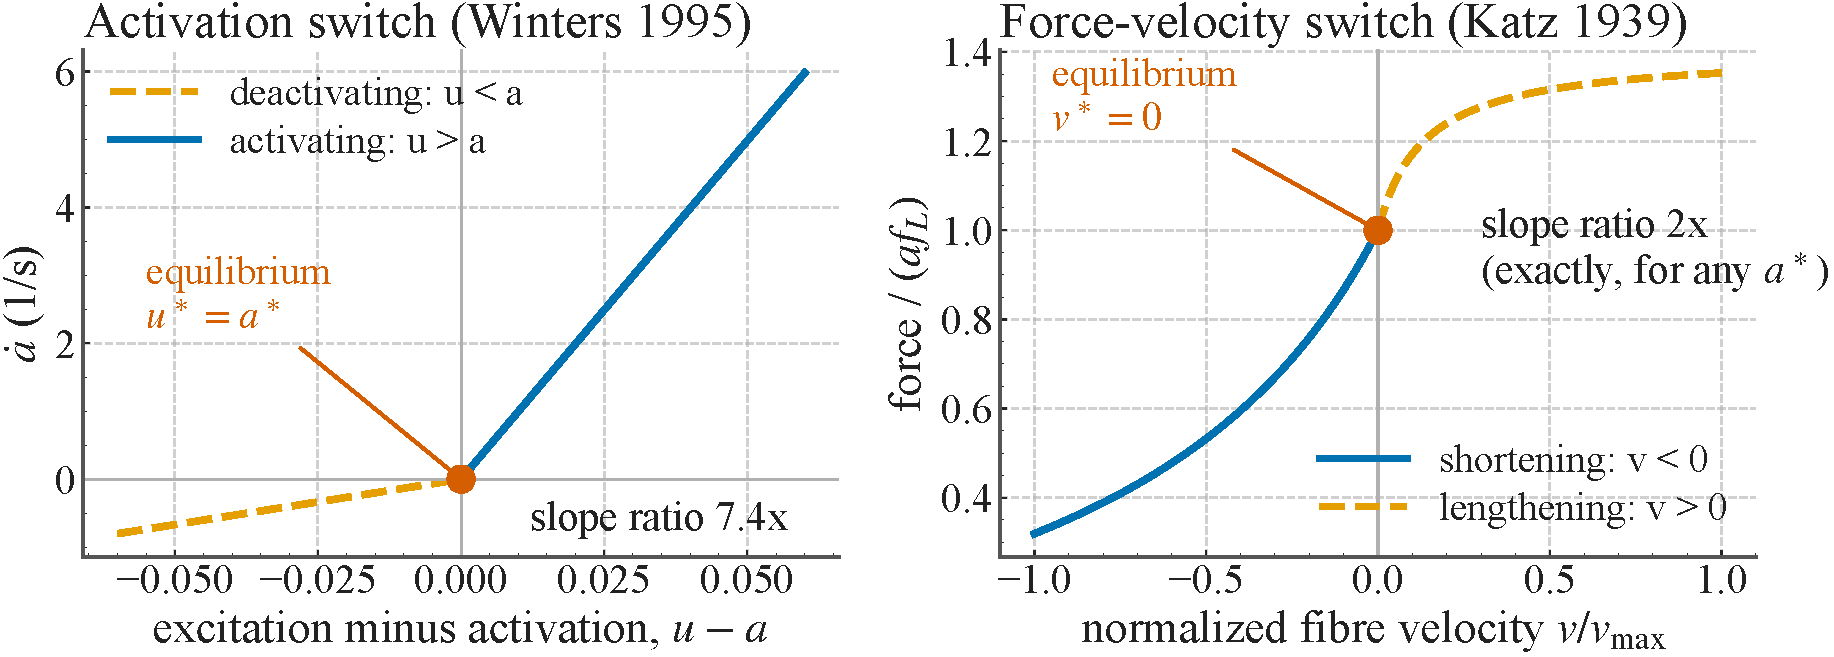
\includegraphics[width=25cm]{fig1_kinks.pdf}};


% The perturbation signs select the directional Jacobian.
\node[draw=accent,fill=accent!5,rounded corners=2mm,labeltext,
  text width=16.5cm,minimum height=3.8cm] (modes) at (9,-2.65)
  {\textbf{Four directional models}\\[.3ex]
  $\{u-a>0,\ u-a\le0\}\ \times\ \{v>0,\ v\le0\}$\\[.3ex]
  $\delta\dot x=A_i\delta x+B_i\delta u$};
\node[draw=accent,fill=accent!5,rounded corners=2mm,labeltext,
  text width=15.3cm,minimum height=3.8cm] (mpc) at (29.6,-2.65)
  {\textbf{Update the prediction model}\\[.3ex]
   Measured state $\to$ active branch $\to$ MPC\\[.3ex]
   Test prediction and tracking transients};
\draw[arrow] (modes.east)--(mpc.west);
\end{tikzpicture}

\caption{Project overview: a muscle-driven joint sits on two switching surfaces.
The perturbation selects one of four local models; branch-aware MPC updates
its prediction at the measured state. Elbow drawing is schematic.}
\end{figure}
\end{block}

\begin{block}{\chip{3} Related work}
\textbf{Hill-type modelling.} Thelen models activation and force generation;
Millard et al.\ characterize computational muscle formulations [1,2].

\textbf{Smoothing.} Kirsch et al.\ smooth torque--velocity dynamics; De Groote
et al.\ smooth activation for optimization [3,4]. Here we measure the cost of
branch choice at equilibrium.

\textbf{Non-smooth systems.} Camlibel et al.\ give continuity conditions for
bimodal linear systems [5]. Yeo et al.\ study a distinct force--length
instability, rather than the activation-switch control problem [6].
\end{block}

\begin{block}{\chip{4} Formulation / model}
A forearm--hand pendulum is driven by a rigid-tendon Hill-type brachialis
model: Thelen activation dynamics [1], Holzbaur muscle parameters [7], and
moment arms digitized from Murray et al.\ [8].
\[
 x=[\theta,\dot\theta,a]^{\mathsf T},\qquad
 I\ddot\theta=F^{MT}r(\theta)-mgl_c\sin\theta,\qquad
 v=-\frac{r(\theta)\dot\theta}{l_0^M}.
\]
\[
 \dot a=\frac{u-a}{\tau_a},\qquad
 \tau_a=\begin{cases}
 \tau_{\rm act}(0.5+1.5a),&u>a,\\
 \tau_{\rm deact}/(0.5+1.5a),&u\le a.
 \end{cases}
\]
At $\theta^\ast=60$\dg\ and $a^\ast=0.113$, all four branches are stable.
Each switch satisfies $A_1-A_2=ec^{\mathsf T}$ and $B_1-B_2=ed$ [5]; the
switches affect different Jacobian entries.

\textbf{Strength check:} the three elbow flexors peak at 73.6\,\Nm\ at 94\dg,
against 79\,\Nm\ at 100\dg\ in one measured data set (RMS difference
3.6\,\Nm). This is a simulation study; hardware validation remains open.
\end{block}
\begin{alertblock}{\chip{9} Conclusion}
\textbf{Choose the branch as well as the operating point.}
Directional linearizations matter for prediction and transient control.
Relinearize at the measured state, avoid central differences across a kink,
and compensate delay. Co-contraction can reduce the velocity kink.

\aside{Limits: one simulated joint; no reflexes, short-range stiffness or
history dependence. Tracking rankings depend on controller weights and noise.}
\end{alertblock}

\begin{exampleblock}{References}
{\small
[1] Thelen DG (2003). \emph{J Biomech Eng} 125:70--77.\quad
[2] Millard M et al.\ (2013). \emph{J Biomech Eng} 135:021005.\par
[3] Kirsch NA et al.\ (2018). \emph{IEEE TNSRE} 26:224--232.\quad
[4] De Groote F et al.\ (2016). \emph{Ann Biomed Eng} 44:2922--2936.\par
[5] Camlibel MK et al.\ (2008). \emph{Automatica} 44:1261--1267.\quad
[6] Yeo SH et al.\ (2023). \emph{J R Soc Interface} 20:20220430.\par
[7] Holzbaur KRS et al.\ (2005). \emph{Ann Biomed Eng} 33:829--840.\quad
[8] Murray WM et al.\ (1995). \emph{J Biomech} 28:513--525.\par}
\end{exampleblock}
\end{column}
\separatorcolumn
\begin{column}{\colwidth}

\begin{block}{\chip{5} Results: prediction error}
A $+0.01$ excitation step at the reference posture separates the four local
predictions. At 50\,ms, the matched model errs by \hi{1.1\%} of the true swing;
the wrong activation, velocity and combined branches err by
\hi{71\%, 14\% and 75\%}, respectively.
\begin{figure}
\centering
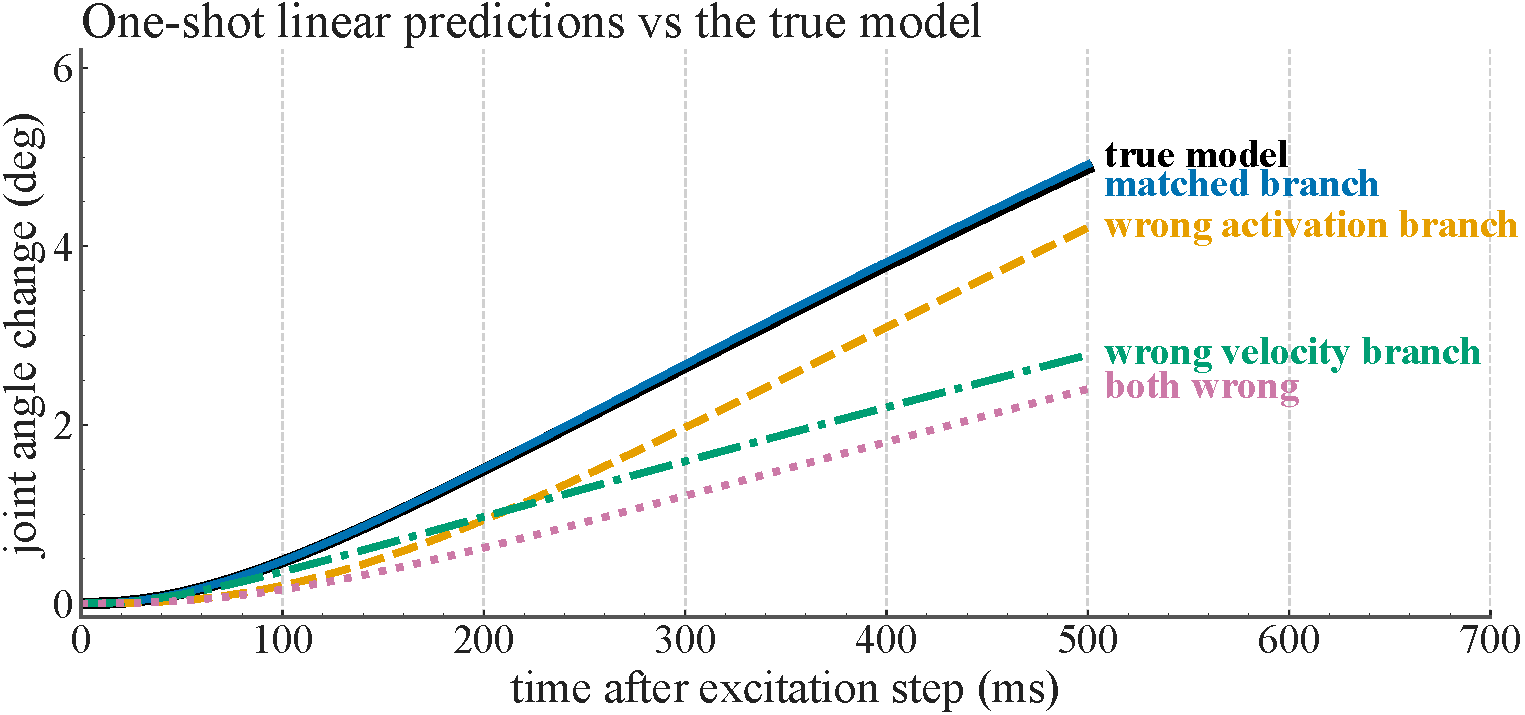
\includegraphics[width=0.70\linewidth]{fig2_prediction.pdf}
\caption{Only the matched branch closely tracks the nonlinear response.}
\end{figure}
\end{block}

\begin{block}{\chip{6} Results: across operating points}
With both branches wrong, error is \textbf{at least 23\% of the activating-step
signal} at every single-muscle equilibrium tested.
\begin{figure}
\centering
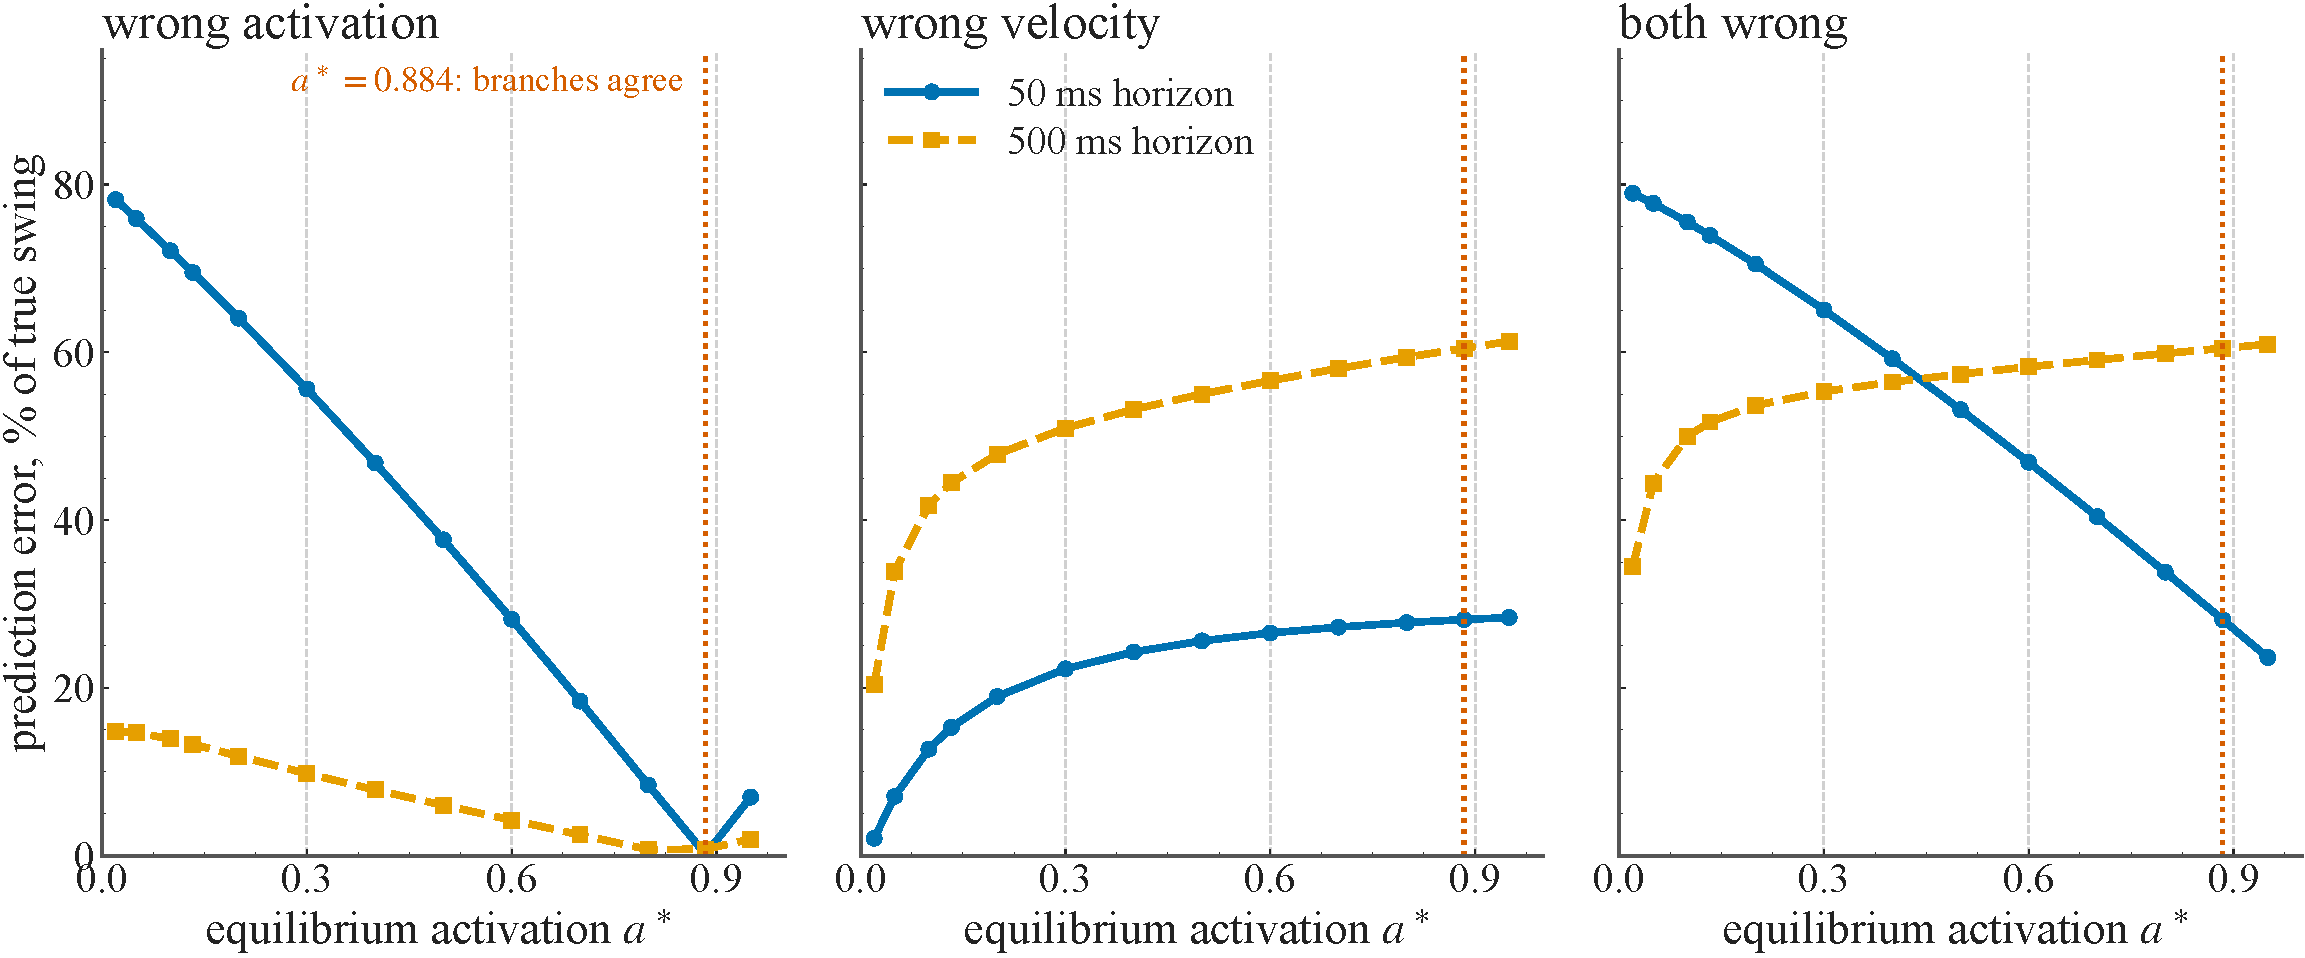
\includegraphics[width=0.70\linewidth]{fig3_equilibria.pdf}
\caption{Held-load sweep at 60\dg: activation-branch error falls as the
velocity-branch error grows. The combined error never vanishes in the sweep.}
\end{figure}
\end{block}

\begin{block}{\chip{7} Results: what survives feedback}
MPC uses identical weights, $N=20$ and $T_s=10$\,ms. Blending the branches gives
\textbf{8--9$\times$ more raising overshoot} than the naive, sign-test and
relinearizing rules. Updating the model cuts lowering overshoot from
\hi{0.37\dg\ to 0.02\dg}.
\begin{figure}
\centering
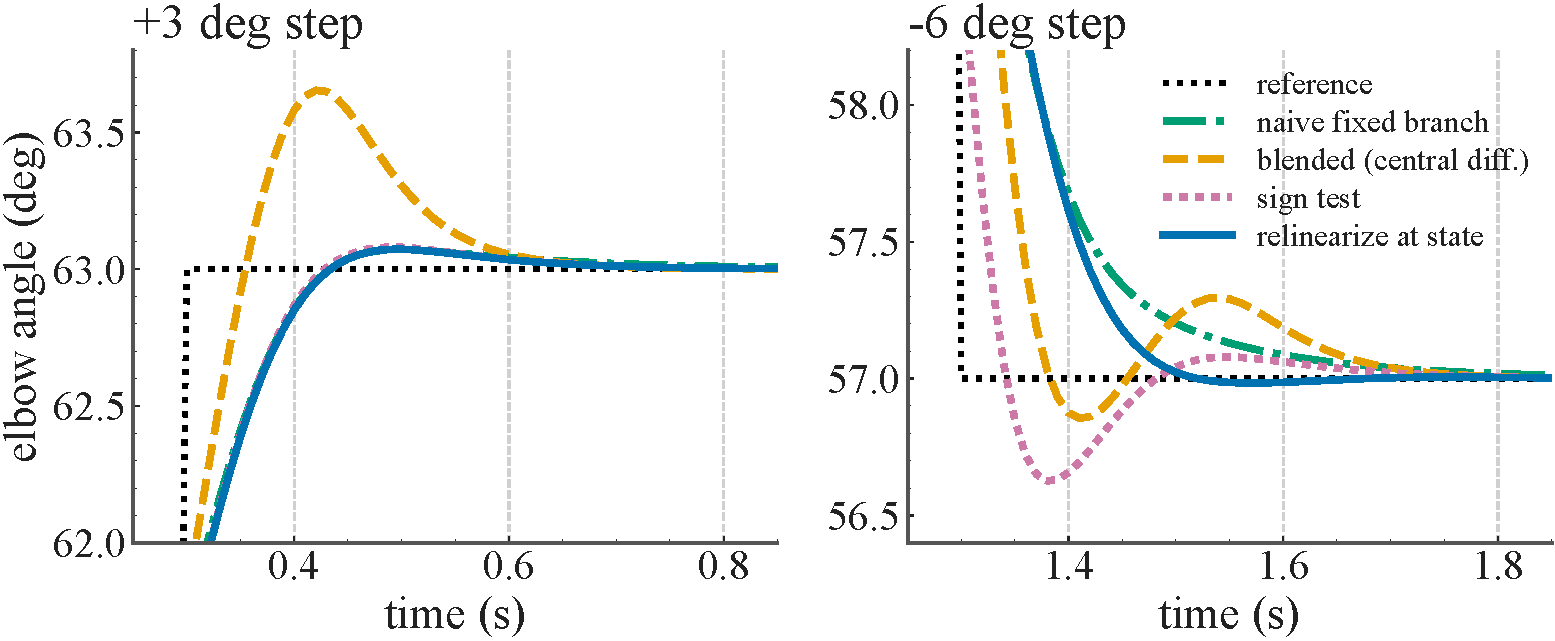
\includegraphics[width=0.70\linewidth]{fig4_closedloop.pdf}
\caption{Tracking 60 $\to$ 63 $\to$ 57\dg. Branch selection affects transients
even when delay-free feedback preserves stability and steady-state tracking.}
\end{figure}
\end{block}

\begin{block}{\chip{8} Results: antagonist co-contraction}
Adding triceps creates \textbf{three switches and eight modes}.
Co-contraction can balance the muscles' directional damping and cancel the
joint velocity kink; the cancellation depends on the moment arms.
\begin{figure}
\centering
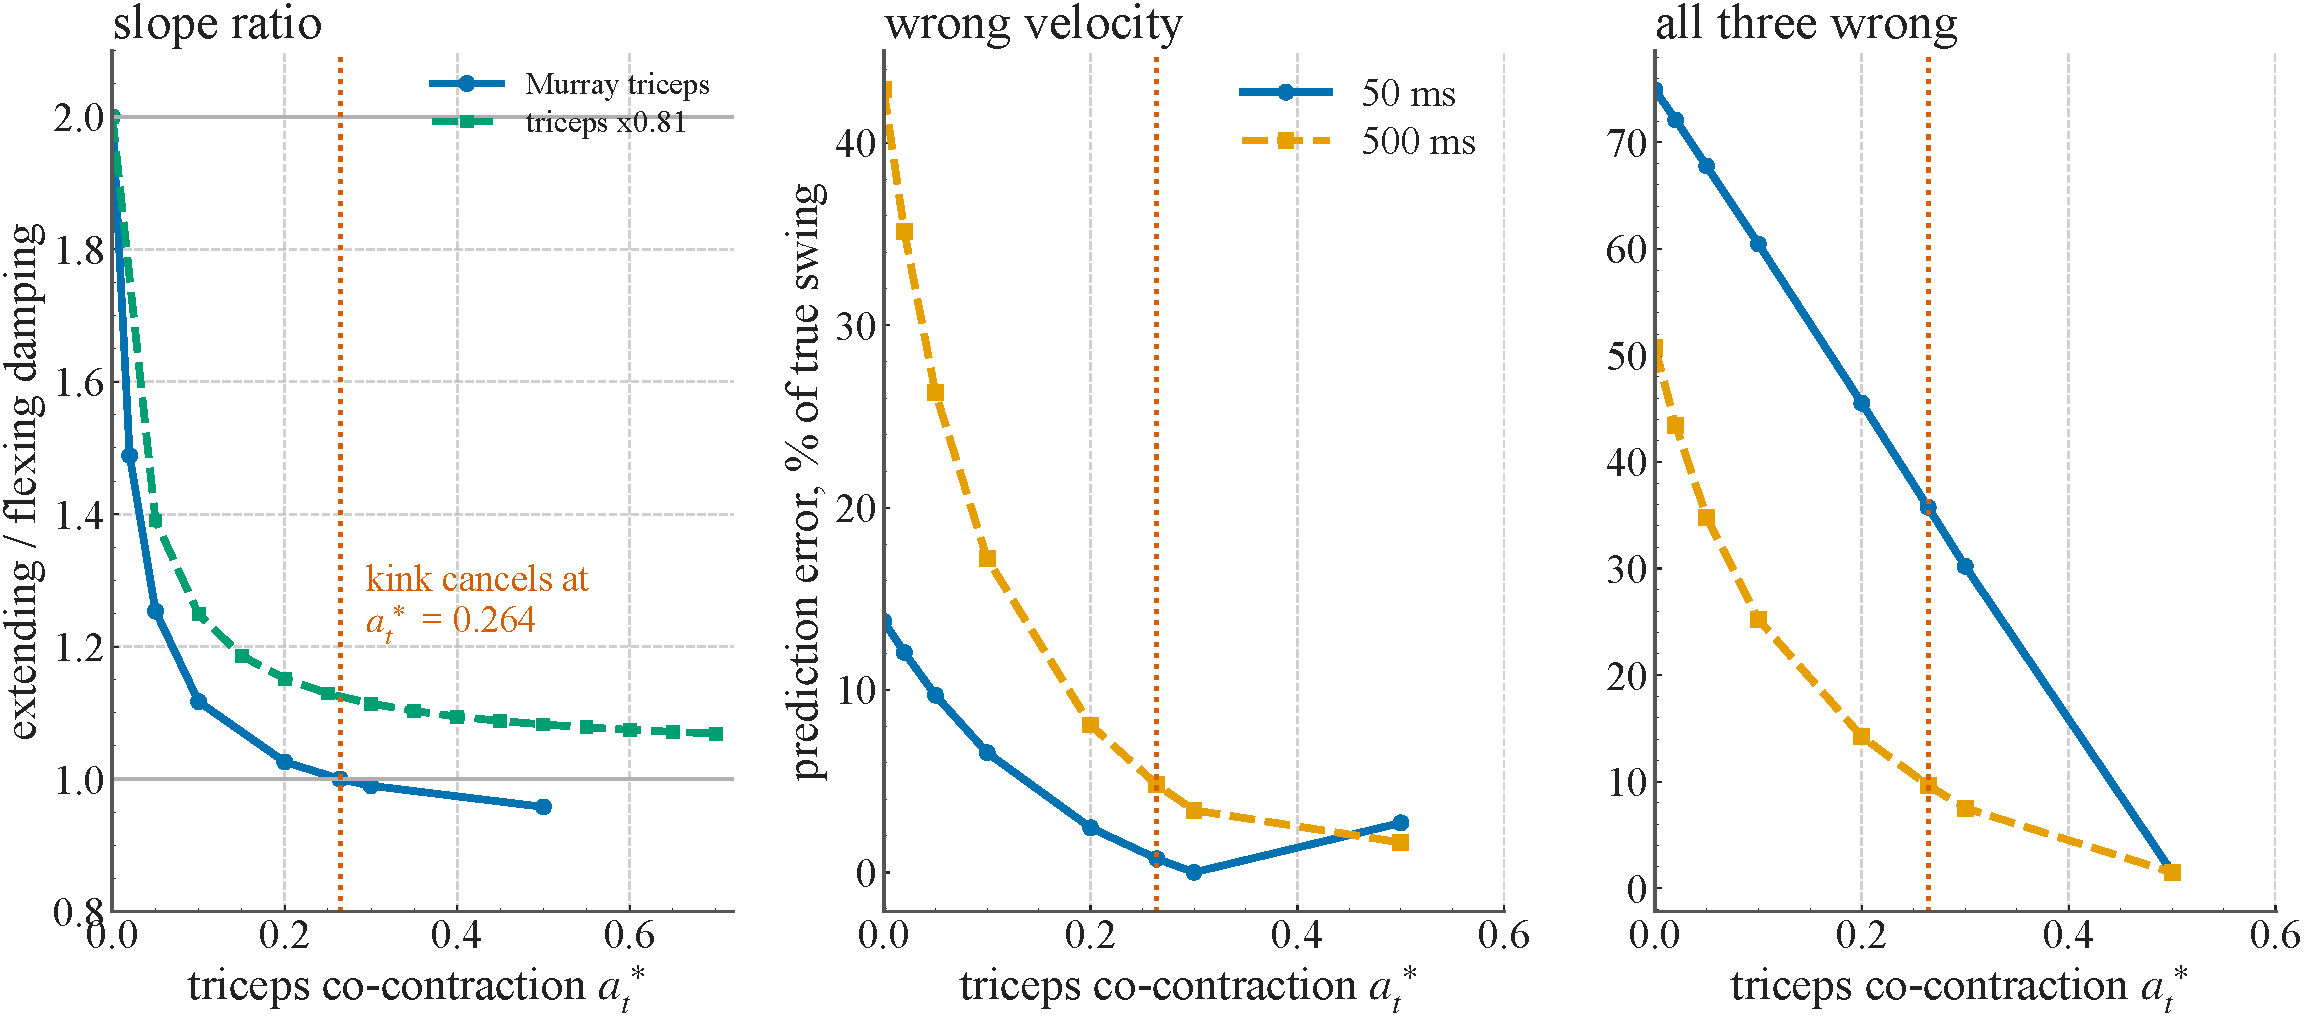
\includegraphics[width=0.70\linewidth]{fig5_pair.pdf}
\caption{ICRA antagonist study at 60\dg. Co-contraction reduces the velocity
slope ratio toward one and reduces wrong-branch errors, at higher effort.}
\end{figure}
\end{block}
\end{column}
\separatorcolumn
\end{columns}
\end{frame}
\end{document}
